\documentclass[a4paper,12pt]{article}

% don't forget the document class, generally : \documentclass[a4paper,12pt]{article}

\usepackage[utf8]{inputenc}
\usepackage[french]{babel}
\usepackage{graphicx}
\usepackage{gensymb}
\usepackage{amsmath}
\usepackage{float}
\usepackage{scrextend}
\usepackage{caption} 
\usepackage{siunitx}
\usepackage{enumitem}
\usepackage{amsthm}
\usepackage{fancyhdr}
\usepackage{amssymb}
\usepackage{wrapfig}
\usepackage{geometry}
\usepackage{standalone}
\usepackage{import}
\usepackage[usenames, dvipsnames]{color}

 \usepackage{biblatex} % manages bibliography and references
\addbibresource{sample.bib}


\geometry{hmargin=1in, vmargin=1in}

 \newenvironment{absolutelynopagebreak}
 {\par\nobreak\vfil\penalty0\vfilneg
 \vtop\bgroup}
 {\par\xdef\tpd{\the\prevdepth}\egroup
 \prevdepth=\tpd}
 
 \pagestyle{fancy}                        
\fancyhf{}                               
\fancyhf[HL]{Application des maths}                
\fancyhf[HR]{Géométrie euclidienne}             
\fancyhf[FC]{\thepage/\pageref{Lastpage}}
 
\newtheorem{definition}{Définition}[section]
\newtheorem{theorem}{Théorème}
\newtheorem{corollary}{Corollaire}[theorem]
\newtheorem{lemma}[theorem]{Lemme}
\newtheorem*{hyp}{Hypothèse}
\newtheorem*{concl}{Conclusion}
\newtheorem*{remark}{Remarque}

\captionsetup{format=default,labelformat=simple,labelsep=colon,
justification=justified,font={sf,small},labelfont=bf,
textfont=default} 



\begin{document}

\pagebreak
\subsection{Théorème du segment moyen}
\begin{theorem}
Une droite passant par les milieux de deux côtés d'un triangle et parallèle au troisième côté de celui-ci.
\end{theorem}

\begin{proof}
Nous considérons le triangle $ABC$ et nous nommons $M$ et $N$ respectivement les milieux des côtés $a$ et $b$. 

 \begin{figure}[H]
        \centering
        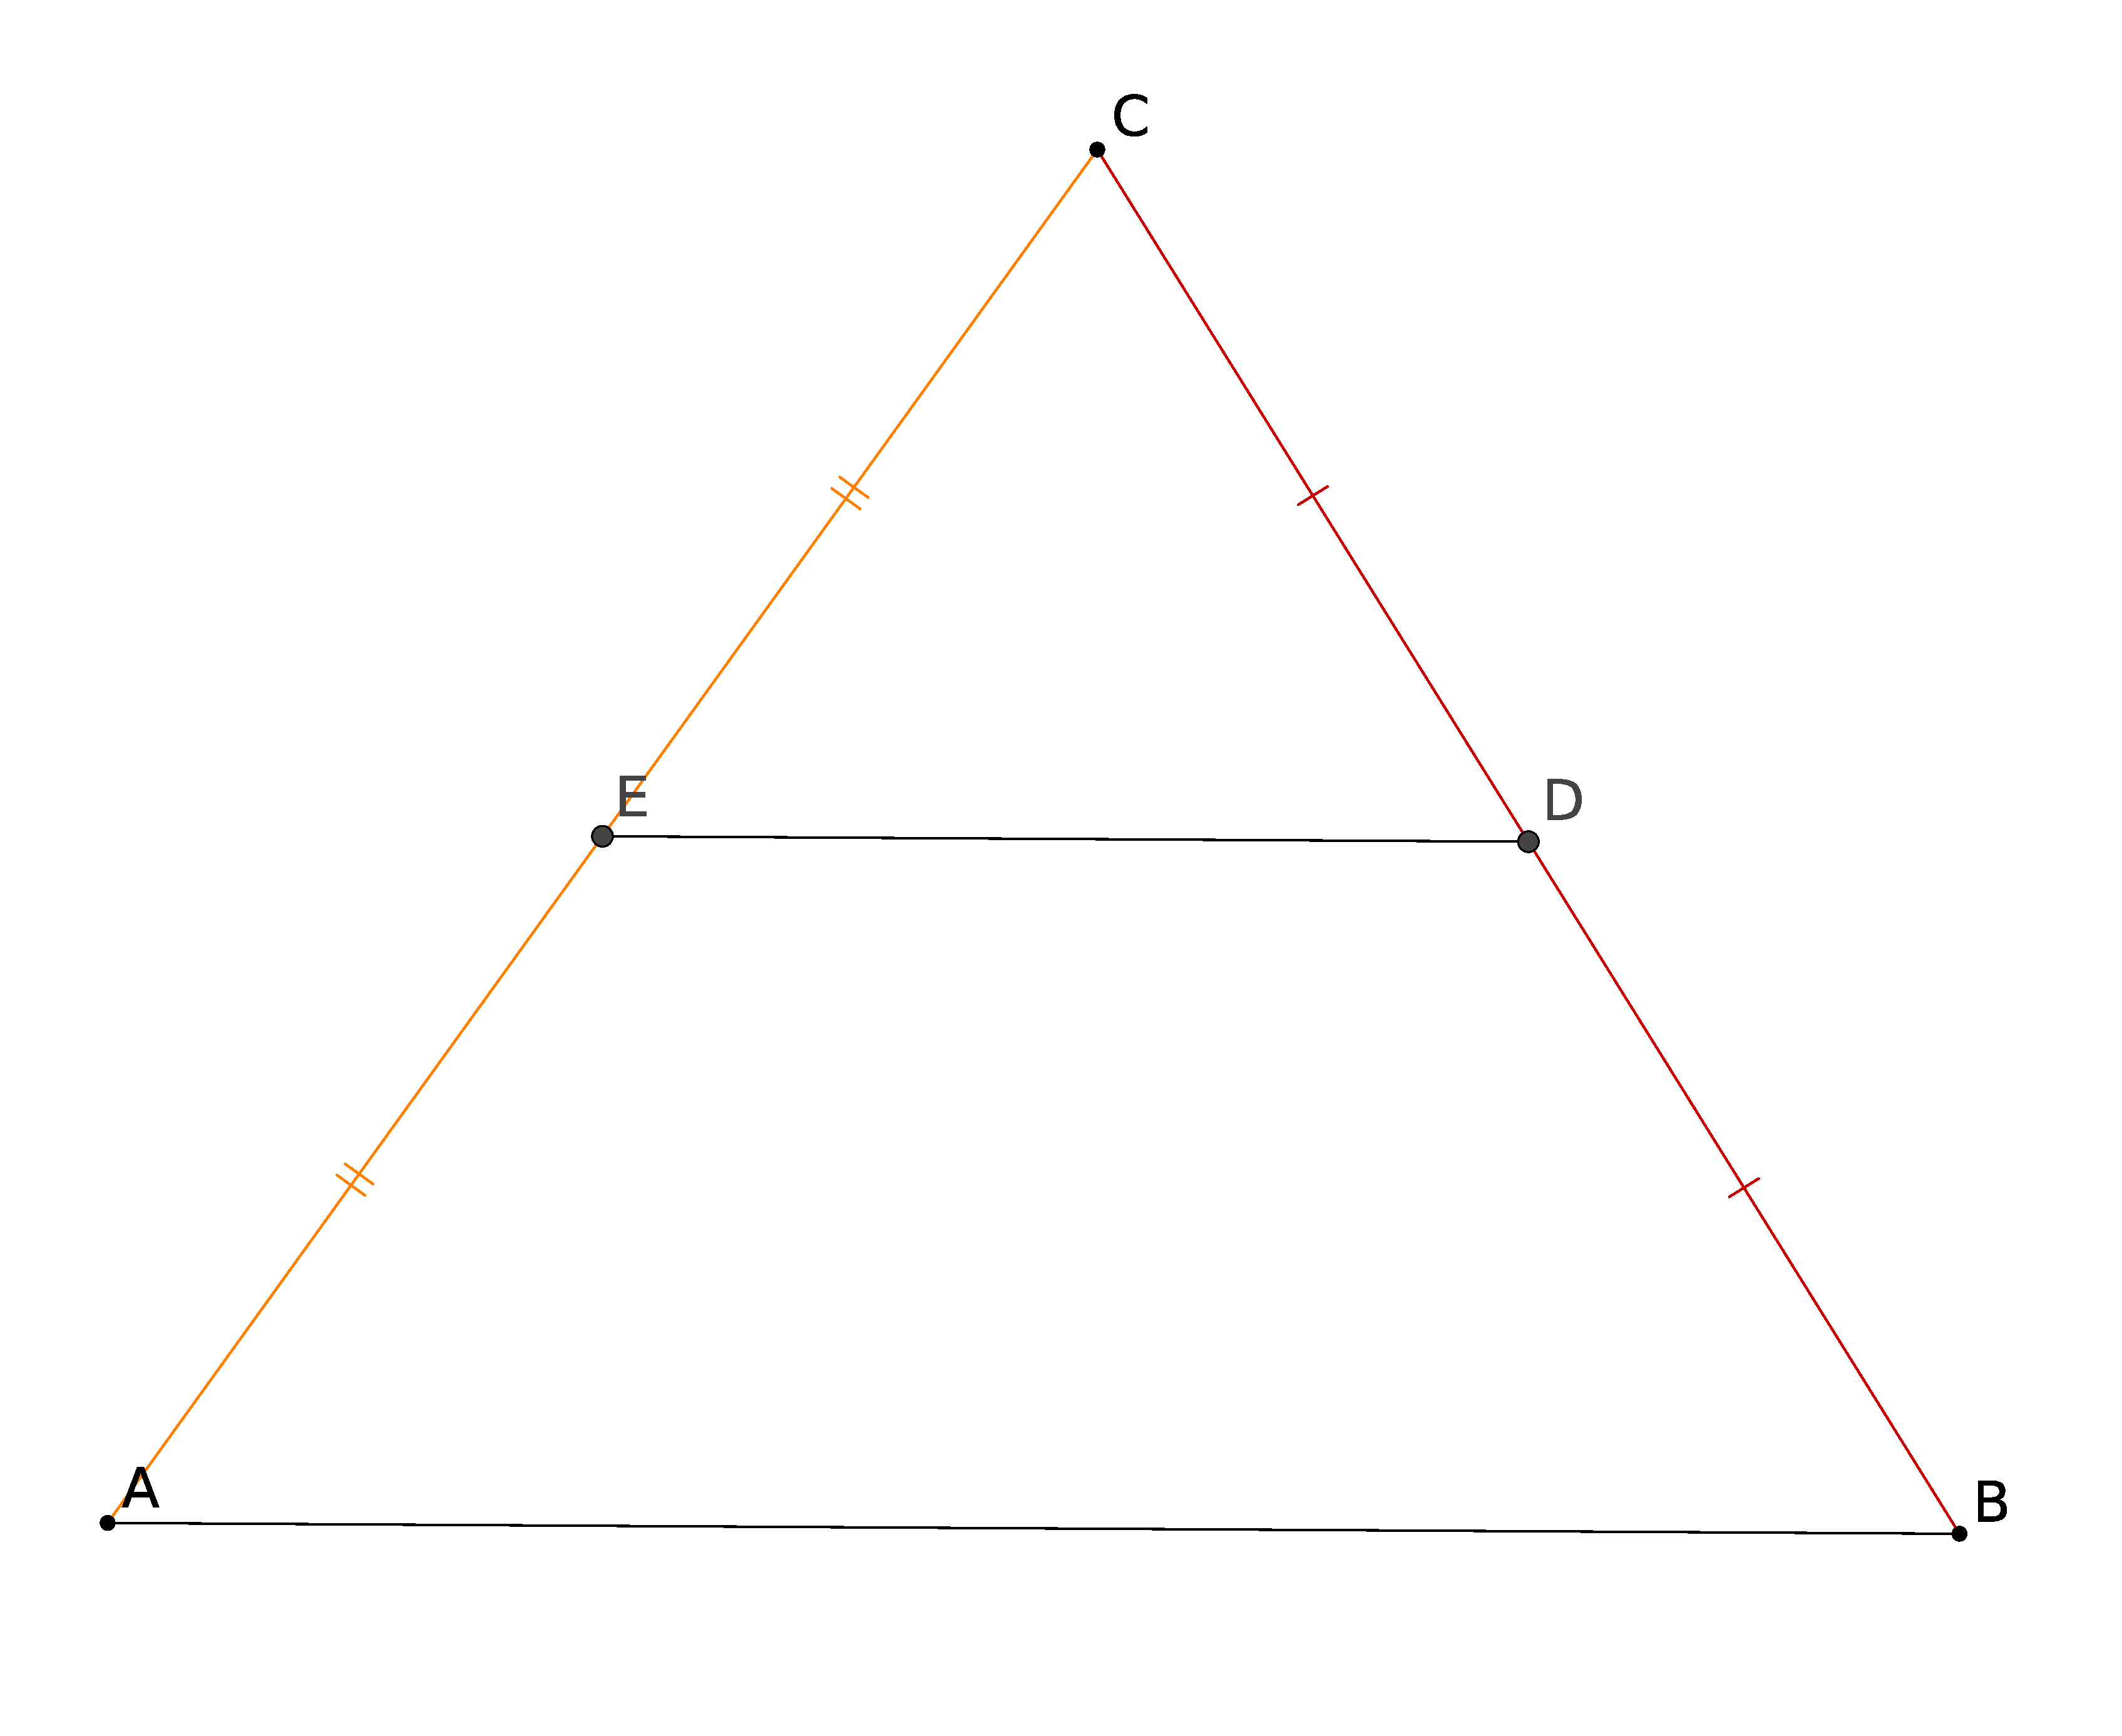
\includegraphics[scale=0.2]{segmentMoyen1.eps}
    \end{figure}

\begin{hyp}
$AM \equiv MC$, $BM \equiv NC$
\end{hyp}

\begin{concl}
$AB \parallel MN$
\end{concl}

Nous commençons par construire un point $P$ sur le prolongement de $MN$ et pour que $PM \equiv MN$. On observe alors que $PANC$ est un parallélogramme, car par construction ses diagonales se coupent en leurs milieux ($PM \equiv MN$ et $AM \equiv MC$).\\

\begin{figure}[H]
        \centering
        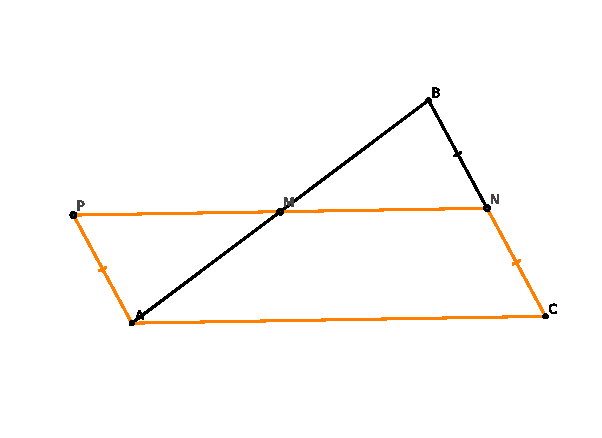
\includegraphics[scale=1.3]{segmentMoyen2.eps}
    \end{figure}

Ensuite, nous pouvons démontrer que le quadrilatère $PANB$ est aussi un parallélogramme, car $PA$ est parallèle et isométrique à $NB$. EN effet, $NB$ est le prolongement de $CN$, qui est parallèle et isométrique à $PA$, ainsi $PA \equiv CN \equiv NB$ (par hypothèse). 

\begin{figure}[H]
        \centering
        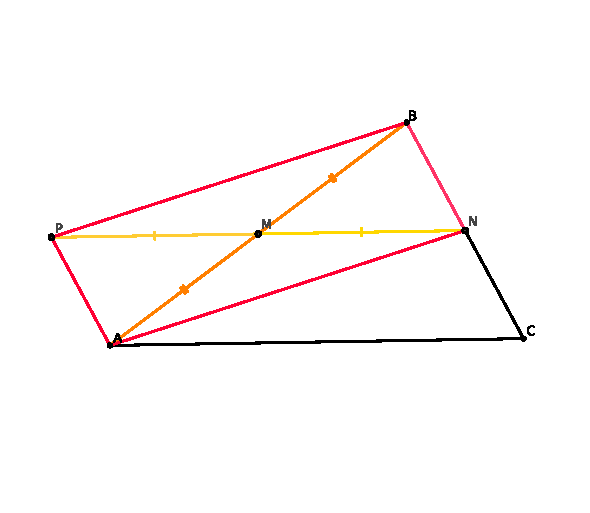
\includegraphics[scale=1.3]{segmentMoyen3.eps}
    \end{figure}

Puisque les segments $PA$ et $NB$ sont isométriques et parallèles, le quadrilatère $PABN$ est un parallélogramme (propriété des parallèlogrammes) et comme ceux-ci ont comme particularité deux paires de côtés parallèles, l'on conclu que $MN \parallel AB$.


\end{proof}




\end{document}